\section{Partition Coloring Problem}

Let $G = (V, E)$ be a non-directed graph and $V$ partitioned into $q$ subsets $V_1, V_2,\ldots, V_q$, where $V_i \cap V_j = \emptyset, \forall i, j = 1, \ldots , q$, $i \neq j$. We refer to $V_1, V_2, \ldots , V_q$ as the components of the partition. The PCP consists in finding a subset $V' \subset V$ such that $|V' \cap V_i| = 1, \forall i = 1, \ldots , q$ (i.e., $V'$ contains one node of each component $V_i$), and the chromatic number of the graph induced in $G$ by $V'$ is minimum.\\
Figure \ref{pd:pcpExample} shows an example of an instance with $10$ nodes and a density of about $0.2$, where density is defined as the probability for each pair of nodes being connected by an edge.

\begin{figure}
\begin{center}
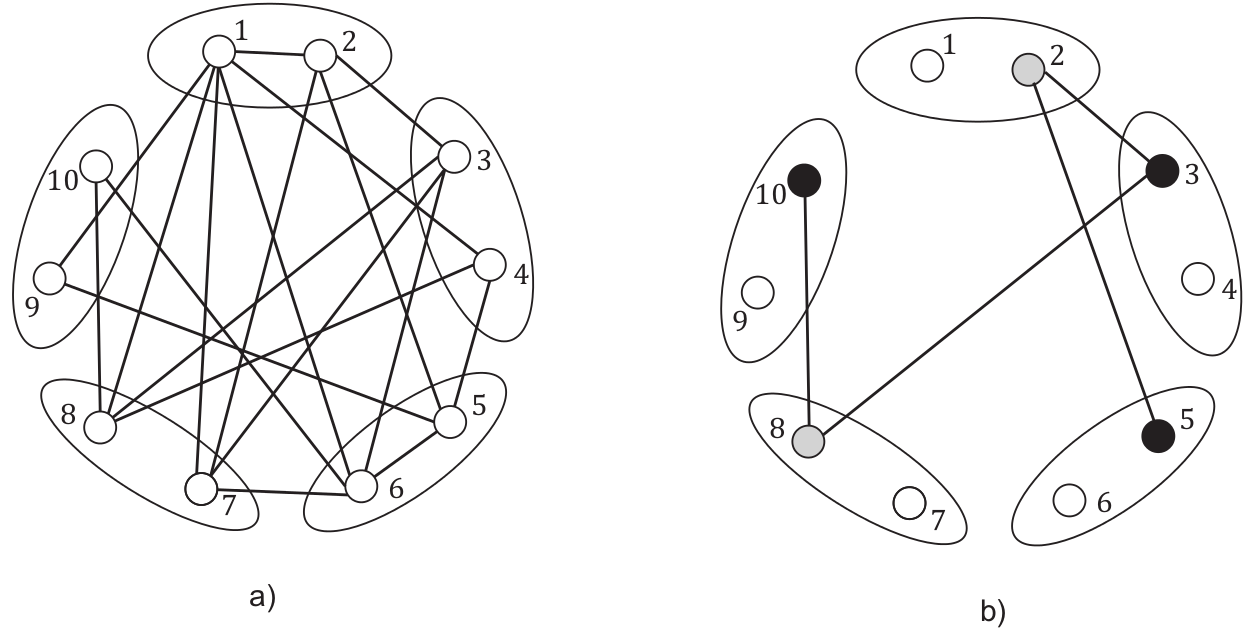
\includegraphics[scale=0.3]{figures/pcp.png}
\caption{(a) Shows a problem instance and (b) its solution.}
\label{pd:pcpExample}
\end{center}
\end{figure}


\section{Wavelength Routing and Assignment Problem}

The PCP has initially been considered by Li and Simha in \cite{li-00} and arises from considering the join problem of routing and wavelength assignment in WDM (Wavelength Division Multiplexing) optical networks. 

%The RWA problem takes two forms: static and dynamic
%[1]. In the static case, all connection requests are known in
%advance, thus a routing decision can be made based on the
%complete knowledge of the traffic to be served by the
%network. The static RWA problem is found to be NP-
%complete that cannot be solved exactly in a polynomial
%T
%This paper resulted from the research supported by the Serbian
%Ministry of science and technological development (project TR-11013).
%Goran Z. Marković is with the Faculty of Traffic and Transport
%Engineering, University of Belgrade, Serbia, Vojvode Stepe 305, 11000
%Belgrade, Serbia; (e-mail:g.markovic@sf.bg.ac.rs).
%Vladanka S. Aćimović-Raspopović is with the Faculty of Traffic and
%Transport Engineering, University of Belgrade, Serbia, Vojvode Stepe
%305, 11000 Beograd, Serbia; (e-mail:v.acimovic@sf.bg.ac.rs).
%time. In the dynamic case, a connection request has to be
%routed and wavelengths assigned independently of other
%connections, which either have already been assigned or
%will be assigned [1]-[3]

\section{Complexity}

%

% -- min-RWA --
%Erlebach and Jansen [7] showed that min-RWA
%is NP-hard. Several authors proposed different
%approximate algorithms for solving min-RWA.
%Banerjee and Mukherjee [4], Hyytia
% ̈ and Virtamo
%[10], and Li and Simha [12] decompose the prob-
%lem in two phases. In the first phase, one or more
%possible routes are computed for each lightpath,
%while in the second one route and one wavelength
%are assigned to each lightpath. The second phase is
%often solved as a colouring problem defined on a
%conflict graph. Manohar et al. [13] proposed the
%Greedy-EDP-RWA construction which was used
%in a multi-start procedure heuristic, in which both
%subproblems are solved simultaneously. Their
%algorithm is much faster and finds solutions as
%good as those found by the algorithm in [4].

